% Chapter Template

\chapter{SCgPC and HDMR for Neutron Transport} % Main chapter title

\label{ch:c5g7} % Change X to a consecutive number; for referencing this chapter elsewhere, use \ref{ChapterX}

\lhead{Chapter 7. \emph{C5G7 Neutronics}} % Change X to a consecutive number; this is for the header on each page - perhaps a shortened title

%----------------------------------------------------------------------------------------
%	SECTION: INTRO
%----------------------------------------------------------------------------------------

\section{Introduction}
The analytic models used in chapters \ref{ch:results scgpc} and \ref{ch:results hdmr} are useful to
analyze the behavior of the stochastic collocation for generalized polynomial chaos (SCgPC) and high-dimension model
representation (HDMR)  methods.  Because they have simply-derived analytic expressions for statistical moments, convergence
and behavior can be analyzed to a high degree of accuracy.  Analytic demonstrations for SCgPC and HDMR have
provided insight regarding when these methods converge quickly, and when they fail to perform better than
traditional Monte Carlo (MC). In practice, however, the models on which we seek to apply
advanced uncertainty quantification methods are seldom analytic.  The response is often solved using nonlinear,
iterative methods, and often involves many different physics in a single calculation.

In the next several chapters, we explore application of advanced uncertainty quantification methods to
engineering-scale performance codes.  In this chapter, we consider a well-understood problem with
relatively few physics, but without an analytic solution.  For this demonstration, we make use of a neutronics
problem.  Neutronics deals with the population and transport of neutrons through some geometry of materials
using the Boltzmann neutron transport equation \cite{lewistrans}. This model is selected for demonstration
because it is more complex than the analytic models, in that there is not a simple analytic expression for the
statistical moments of the responses.  However, the model is still a single integro differential equation, and
contains no direct nonlinearities in its input terms.  This allows some clear analysis despite lack of
analyticity.

\subsection{Neutron Transport}
Neutronics is a branch of nuclear engineering that involves the study, simulation, and design of neutral
particle transport, particularly free neutron transport.  The term \emph{free neutron} describes a neutron
that is not bound to a particular nucleus and moves about with some energy.  The fundamental science behind
nuclear engineering is the fission event, where a free neutron interacts with an atomic nucleus in a way that
produces new free neutrons as well as high-energy fission fragments.  The released energy can be converted to
a variety of uses, most particularly the generation of electrical power.

In order to perform neutronics calculations, we desire to determine the number of neutrons traveling through a
plane in the domain in a given period of time.  The field variable used to describe this quantity is the
\emph{angular flux} $\psi(\mathbf{r},E,\mathbf{\hat\Omega},t)$, which should not be confused with $\phi$ used
to describe polynomials in a gPC expansion.  Angular flux generally is dependent on where in the domain it is
quantified, the energy of neutrons considered, the direction of neutron travel, and time.  

The controlling
equation that approximates neutron transport is the Boltzmann transport equation \cite{duderstadt}
The Boltzmann equation is used to develop a balance equation for neutron conservation as in Eq. 
\ref{eq: neutron trans}.  In this equation, the time rate of change in the angular flux is balance on the left
hand side by removal terms and on the right by source terms.  Removal terms include neutrons traveling out
of a differential area $d\mathbb{r}$, and neutrons interacting with nuclei which potentially changes their
position, energy, direction of travel, or free state.  Source terms include new neutrons produced because of
fission events, neutrons scattering from other directions of travel or energies into the direction of travel
and energy of consideration, new neutrons emitted because of delayed precursors (or post-fission radioactive
nuclei emitting neutrons), and other unspecified sources such as neutrons entering from outside the domain.
\begin{align}\label{eq: neutron trans}
  \qty(\frac{1}{v(E)}\pdv{}{t} + \mathbf{\hat\Omega}\cdot\nabla +
   \Sigma_t(\mathbf{r},E,t))&\psi(\mathbf{r},E,\mathbf{\hat\Omega},t) =
  \frac{\chi_p(E)}{4\pi}\intzf \nu\Sigma_f(\mathbf{r},E',t)\phi(\mathbf{r},E',t)\ dE' \nonumber \\
  & + \int\limits_{4\pi}^{}\intzf \Sigma_s(\mathbf{r},E'\to E,\mathbf{\hat\Omega'\to\hat\Omega},t)
  \psi(\mathbf{r},E',\mathbf{\hat\Omega'},t)  \ dE'\ d\Omega' \nonumber \\
  & + \sum_{i=1}^I \frac{\chi_{d,i}(E)}{4\pi}\lambda_iC_i(\mathbf{r},t) \nonumber \\
  & + s(\mathbf{r},E,\mathbf{\hat\Omega},t),
\end{align}
where
\begin{itemize}
  \item $\mathbf{r}$ is location in three-dimensional space,
  \item $E$ is neutron energy,
  \item $\mathbf{\hat\Omega}$ is a unit vector solid angle parallel to neutron velocity,
  \item $t$ is time,
  \item $v(E)$ is the magnitude of the neutron velocity,
  \item $\psi(\mathbf{r},E,\mathbf{\hat\Omega},t)$ is the \emph{angular flux},
  \item $\phi(\mathbf{r},E,t)$ is the integral of $\psi$ over angle (\emph{scalar flux}),
  \item $\nu$ is the average number of neutrons produced per fission,
  \item $\chi_p(E)$ is the probability distribution function for neutrons produced by fission,
  \item $\chi_{d,i}(E)$ is the probability distribution function for neutrons with energy $E$ produced by
    delayed neutron precursors,
  \item $\Sigma_t(\mathbf{r},E,t)$ is the macroscopic total interaction cross section,
  \item $\Sigma_f(\mathbf{r},E',t)$ is the macroscopic fission cross section,
  \item $\Sigma_s(\mathbf{r},E'\to E,\mathbf{\hat\Omega'\to\hat\Omega},t)$ is the macroscopic scattering cross
    section for neutrons scattering from energy $E'$ to energy $E$ and from solid angle trajectory
    $\mathbf{\hat\Omega'}$ to $\mathbf{\hat\Omega}$,
  \item $I$ is the number of delayed neutron precursors,
  \item $\lambda_i$ is the decay constant for precursor $i$,
  \item $C_i(\mathbf{r},t)$ is the total number of precursor $i$ in $d\mathbf{r}$ at time $t$,
  \item $s(\mathbf{r},E,\mathbf{\hat\Omega},t)$ is an arbitrary source term,
\end{itemize}
and we assume
\begin{itemize}
  \item free neutrons have no interaction with other free neutrons,
  \item total and fission cross sections are assumed angularly independent,
  \item fission neutrons are emitted isotropically after fission events, and
  \item delayed neutrons are emitted isotropically after precursor decay.
\end{itemize}
More details about the physical interpretation of these terms can be obtained in \cite{duderstadt},
\cite{lewis}, and \cite{lewistrans}.

One particular application of the neutron transport equation is reactor criticality.  Criticality problems are
chiefly concerned with the sustainability of a neutron reaction in fissionable material.  Given a particular
set of materials in a given geometry, an analyst needs to determine if the number of neutrons is growing over
time, diminishing over time, or remaining constant.  This analysis is performed by reducing the neutron
transport equation (Eq. \ref{eq: neutron trans}) to steady-state operation and introducing the $k$-eigenvalue,
\begin{align}\label{eq: neutron k}
  \qty(\mathbf{\hat\Omega}\cdot\nabla +
   \Sigma_t(\mathbf{r},E))&\psi(\mathbf{r},E,\mathbf{\hat\Omega}) =
   \frac{1}{k}\frac{\chi_p(E)}{4\pi}\intzf \nu\Sigma_f(\mathbf{r},E')\phi(\mathbf{r},E')\ dE' \nonumber \\
  & + \int\limits_{4\pi}^{}\intzf \Sigma_s(\mathbf{r},E'\to E,\mathbf{\hat\Omega'\to\hat\Omega})
  \psi(\mathbf{r},E',\mathbf{\hat\Omega'})  \ dE'\ d\Omega',
\end{align}
where we have removed the precursors and arbitrary source for this population-balancing problem.  The
$k$-eigenvalue is defined such that the following relationship between its value and the reaction
sustainability exists:
\begin{itemize}
  \item If $k > 1$, the number of neutrons is growing in time.
  \item If $k < 1$, the number of neutrons is diminishing in time,
  \item If $k = 1$, the reaction is exactly sustained.
\end{itemize}
For design of commercial nuclear power plants, a $k$-eigenvalue near unity is often desired to maintain balanced
plant operation.

In order to reduce Eq. \ref{eq: neutron k} into a form suitable for numerical application, we discretize
the energy space $E$ into $G$ distinct \emph{energy groups}.  For historical reasons, the energy group with
the highest-energy neutrons are labeled with energy group $g=1$, while the lowest energy neutrons are in group
$g=G$.  This allows integrals to be approximated by sums, and introduces the subscript $g$ to refer to the
energy group for which each term applies.  This discretization generates $G$ equations coupled through the
fission and scattering terms, each with the form
\begin{align}\label{eq: neutron energy}
  \qty(\mathbf{\hat\Omega}\cdot\nabla +
  \Sigma_{t,g}(\mathbf{r}))&\psi_g(\mathbf{r},\mathbf{\hat\Omega}) =
  \frac{1}{k}\frac{\chi_{p,g}}{4\pi}\sum_{g'=1}^G \nu\Sigma_{f,g'}(\mathbf{r})\phi_{g'}(\mathbf{r}) \nonumber \\
  & + \int\limits_{4\pi}^{} \sum_{g'=1}^G \Sigma_{s,g'\to g}(\mathbf{r},\mathbf{\hat\Omega'\to\hat\Omega})
  \psi_{g'}(\mathbf{r},\mathbf{\hat\Omega'}) \ d\Omega',
\end{align}
where cross sections and material properties are taken at their expected value within the energy group, such
as
\begin{equation}
  \Sigma_{t,g} \equiv \int\limits_{E_{g+1}}^{E_{g}} \Sigma_t(\mathbf{r},E')\ dE',
\end{equation}
where $E_g$ is the maximum energy in group $g$ and $E_{G+1}$=0.  By discretizing the energy space, some error
is introduced which is dependent on the number of energy groups $G$.  In coarse problems, often the energy
space is divided into two energy groups: those neutrons with energy less than or equal to equilibrium thermal
neutron energy in the reactor, and those neutrons with greater energy.
In more fine calculations, up to hundreds of energy groups can be used
\cite{lewistrans}.

One dimension that still causes difficulty in Eq. \ref{eq: neutron energy} is the dependence on angular
scattering; that is, there is no limit placed on the distribution dependence of scattered neutrons on the
incident neutron angle.  One approach to this numerical obstacle is to discretize angular space into discrete
solid angles.  This method is referred to as S$_\text{N}$ or discrete ordinates.  If the approximation
is made that scattering is at most linearly anisotropic, the resulting simplification of Eq. \ref{eq: neutron energy}
is the \emph{diffusion} equation \cite{duderstadt},
\begin{equation}\label{eq:diffusion}
  -D_g(\mathbf{r})\nabla^2\phi_g(\mathbf{r}) + \Sigma_{a,g}(\mathbf{r}) =
  \sum_{g'=1}^G \Sigma_{g'\to g}\phi_{g'}(\mathbf{r}) + 
  \frac{\chi_{p,g}}{k}\sum_{g'=1}^G \nu\Sigma_{f,g'}(\mathbf{r})\phi_{g'}(\mathbf{r}),
\end{equation}
where we introduce the diffusion coefficient $D$,
\begin{equation}
  D_g(\mathbf{r}) = \frac{1}{3\Sigma_{t,g}(\mathbf{r})},
\end{equation}
which comes from Fick's first law of diffusion and relates flux in a diffusive problem to steady-state
concentration \cite{lewis}.
Because of integration over angle our field quantity of interest transitions from angular flux
$\psi_g(\mathbf{r},\mathbf{\hat\Omega})$ to \emph{scalar flux} $\phi_g(\mathbf{r})$, defined by
\begin{equation}
  \phi_g(\mathbf{r}) \equiv \int\limits_{4\pi}^{} \psi_g(\mathbf{r},\mathbf{\hat\Omega})\
  d\mathbf{\hat\Omega},
\end{equation}
where we introduce the macroscopic absorption cross section $\Sigma_{a,g}(\mathbf{r})$.  Eq. \ref{eq:diffusion} is
well-suited to solution by numerical means by discretizing the domain mesh and applying a solution scheme such
as finite elements.  In some simple geometries Eq. \ref{eq:diffusion} has analytic solutions.  

We note
that this diffusion approximation is most accurate when the dominant physics is isotropic neutron scattering.  
As a result, it
performs poorly near strong absorbers, transition boundaries between materials, and on the boundaries of the
problem.  As long as the problem has large scattering cross sections and the domain is large with respect to
the neutron mean free path, however, it is a reasonable
approximation to the full neutron transport equation, and is much more conducive to numerical solution.

\section{Problem}
The problem we apply the diffusion equation and our advanced uncertainty quantification techniques is a
benchmark for mixed-oxide (MOX) fuel assemblies in a pressurized water reactor.  This benchmark is
commonly referred to as C5G7 \cite{c5g7}, and specifications are available for both two-dimensional and three-dimensional
geometries.  In our case, we consider the two-dimensional specifications.

\subsection{Physical Problem}
The geometry of this problem consists of a quarter-symmetric miniature core with four assemblies surrounded by
a reflector.  The geometry can be seen in Figure \ref{fig:c5g7 geom}.  In this figure, reflecting boundary
conditions are imposed on the left and bottom, while vacuum boundaries are applied at the top and right.
The mesh is fine triagonal elements, as shown for fuel elements in Figure \ref{fig:c5g7 mesh}, with a coarser
mesh in the moderator.  In Figure \ref{fig:c5g7 geom} we see four assemblies in a two-by-two array surrounded
by a reflector.
Two example scalar flux profiles from the reference input realization can be seen in Figs. \ref{fig:c5g7 flux0} and
\ref{fig:c5g7 flux1}.  Seven materials make up the domain:
\begin{itemize}
  \item UO2, the fuel for the bottom-left and upper-right assemblies;
  \item 4.3\% enriched MOX fuel, the outer fuel for the bottom-right and upper-left assemblies;
  \item 7.0\% enriched MOX fuel, the next-to-outer fuel for the MOX assemblies;
  \item 8.7\% enriched fuel, the innermost fuel for the MOX assemblies;
  \item Guide tubes, interspersed points within the innermost fuel in all assemblies;
  \item Fission chambers, the central point in each assembly; and
  \item Reflector, the material outside the assemblies.
\end{itemize}
Each assembly is comprised of 17 by 17 square pin cells.
Each pin cell is un-homogenized; that is, a pin cell is comprised of either a fuel pin, guide tube, or
fission chamber surrounded by moderator.  The pin cell is 1.26 centimeters on a side, while the radius of the
fuel pin, guide tube, or fission chamber has a radius of 0.54 centimeters.  The cladding and gap for fuel
pins are homogenized into the fuel pin itself.  

We discretize the energy space for this problem into eight energy groups.  
The discrete energy group boundaries are
given in Table \ref{tab:c5g7 energy} \cite{c5g7}.

\begin{figure}[htb]
  \centering
  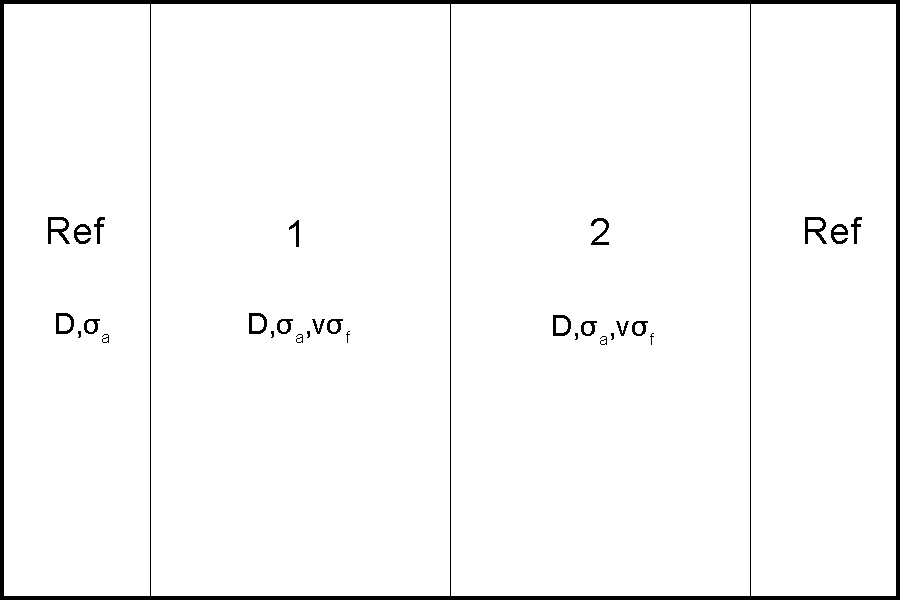
\includegraphics[width=0.7\linewidth]{c5g7/geom}
  \caption{C5G7 Geometry}
  \label{fig:c5g7 geom}
\end{figure}
\begin{figure}[htb]
  \centering
  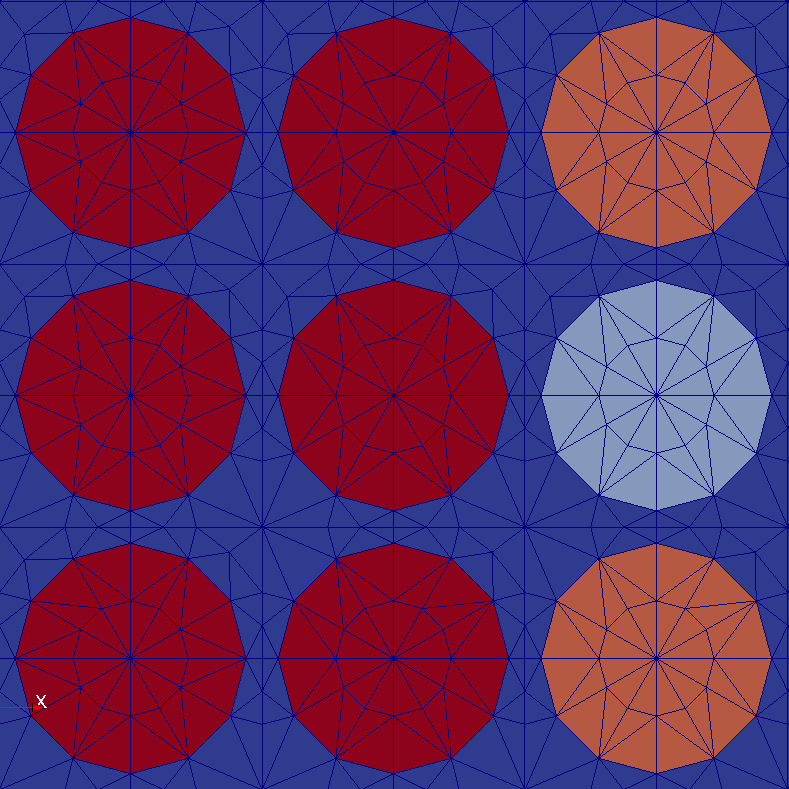
\includegraphics[width=0.7\linewidth]{c5g7/mesh}
  \caption{Partial C5G7 Mesh}
  \label{fig:c5g7 mesh}
\end{figure}
\begin{figure}[htb]
  \centering
  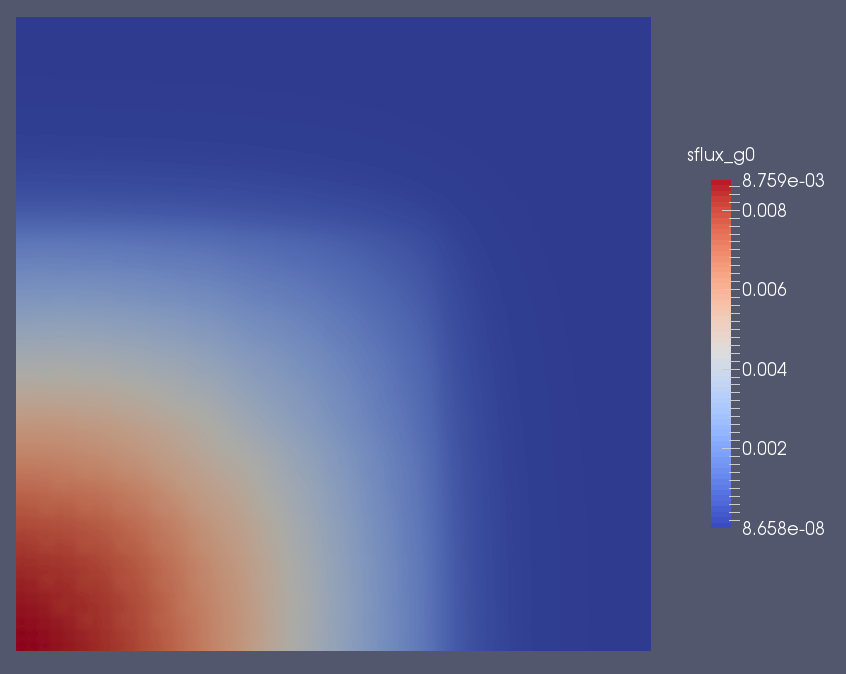
\includegraphics[width=0.7\linewidth]{c5g7/flux0}
  \caption{C5G7 Group 1 (Fast) Flux}
  \label{fig:c5g7 flux0}
\end{figure}
\begin{figure}[htb]
  \centering
  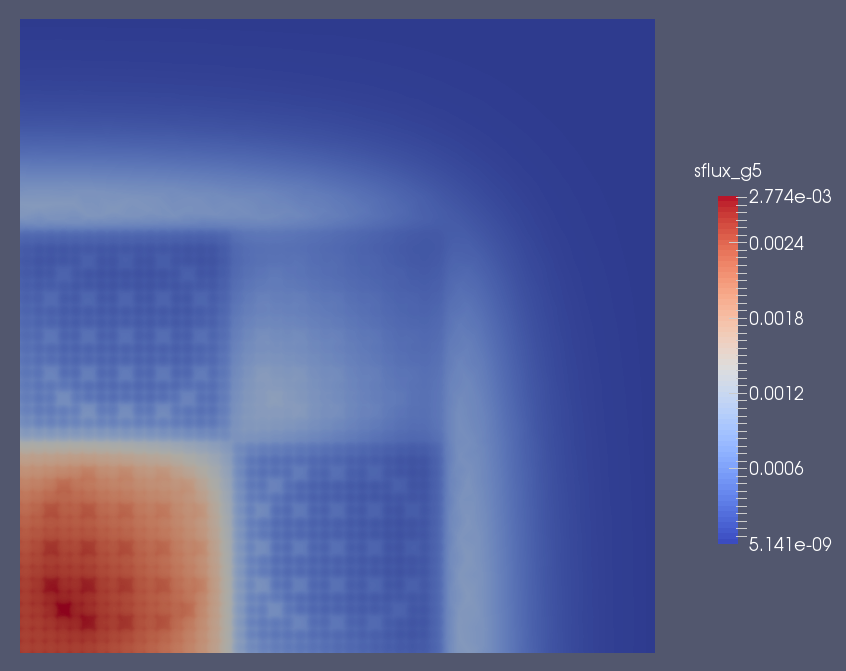
\includegraphics[width=0.7\linewidth]{c5g7/flux5}
  \caption{C5G7 Group 5 (Thermal) Flux}
  \label{fig:c5g7 flux1}
\end{figure}

\begin{table}
  \centering{}
  \begin{tabular}{c c}
    Group & Upper Energy Bound \\ \hline
    7 & 0.02 eV\\
    6 & 0.1 eV\\
    5 & 0.625 eV\\
    4 & 3 eV\\
    3 & 500 keV \\
    2 & 1 MeV \\
    1 & 20 MeV
  \end{tabular}
  \caption{C5G7 Energy Groups}
  \label{tab:c5g7 energy}
\end{table}
This problem is solved using \moose{}-based application \rattlesnake{} \cite{rattlesnake} using the diffusion
equation as the driving physics.  \moose{}-based applications use continuous finite elements for mesh interpolation.  
The flux field parameter is set to use first-order Lagrange polynomials to
interpret the finite element space.  
For this problem the \rattlesnake{} solver parallelizes quite effectively up to six
parallel processes per evaluation. On the Idaho National Laboratory supercomputing framework \texttt{FALCON} each
run takes approximately one minute to converge using \moose{}'s preconditioned Jacobian-free Newton Krylov
solver \cite{moose} when parallelized with six processes.

\subsection{Uncertainty}
There are a total of 168 correlated macroscopic cross sections as uncertain inputs to this problem.  To
introduce uncertainty in these cross sections, we use the nominal reference case cross sections as the mean
values of Gaussian normal distributions, and assign a standard deviation of five percent of the mean to all 
inputs.  We also assign
correlations between cross sections of the same type and material but different energy groups, as well as
correlations between cross sections of the same energy group and material but different types.  The
correlation we assign in either case ten percent.  This results in a symmetric covariance matrix that is sparse with
blocks of nonzero entries.  This approximate covariance matrix could be improved by using uncertainty propagation
on a cross section generation tool to calculate actual covariances; however, for demonstration purposes, we
make use of
these assigned values.

We consider three responses for this model: the $k$-eigenvalue, and the thermal and fast ($g=1,5$) scalar 
flux measured in the center of the
bottom-left element in the mesh, which is near to the center of the reactor.  In order to provide an
orthogonal and reasonably-sized uncertainty space, we first use \raven{} \cite{raven} to perform a Karhunen-Loevre (KL) 
\cite{karhunen}
expansion.  This results in a surrogate input space made up of orthogonal, standard normally-distributed
variables.  We refer to the collection of surrogate input variables as \emph{latent} variables, which are
labeled only by their ranking in the KL expansion.  For example, \texttt{latent\_6} is the sixth dimension in
the KL expansion.  The original input space we designate the \emph{manifest} input space, as these are the
inputs manifested to the simulation model.  This follows the naming convention in \raven{}.

We then perform a sensitivity analysis of the responses to the latent inputs using ten thousand Monte Carlo samples.  
The sensitivity values and KL
eigenvalues are used together to construct an importance index, ranking the impact of each latent variable on
both the input and response spaces.  Importance rank is normalized to one, giving roughly an idea of the
percent of the model retained due to truncation.  The KL expansion and sensitivity ranking, along with importance
determination, are utilities we use in \raven{}'s toolkit \cite{physor2016}.  

The first several importance-ranked eigenvalues
for each response are shown in Table \ref{tab:c5g7 importance}.  There are many latent input dimensions common
in the first several importance rankings for each variable; in particular, latent dimensions 24, 9, 0, and 17
are common to all three, while additionally 10 is common to both the flux terms.  We elect to truncate the
latent input space to include these common terms plus dimension 116 (important to the group 1 flux) and
dimensions 100 and 13 (important to the group 5 flux).  In total this gives our reduced input space a
dimensionality of eight.  This reduction is significant; we only keep 18 percent of the $k$-eigenvalue
importance, and 16 percent of the two flux importance.  

Figures \ref{fig:c5g7 eigenvalue imprank} through
\ref{fig:c5g7 flux 5 imprank} show the importance rank of each response.  The red cross series corresponding
to the left y-axis is the importance of each rank as a function of the ranking itself, as is shown in Table
\ref{tab:c5g7 importance}.  The blue circle series corresponding to the right y-axis is the cumulative
importance rank as a function of the number of dimensions kept in order of rank.  A black line has been added
to indicate at which level each series was truncated.  The flux responses were both truncated at the end of
the steep drop in importance rank values, while the eigenvalue was truncated somewhat more than that.  Despite
this steep truncation, we see much of the original response preserved.

\begin{table}
  \centering
  \begin{tabular}{|c|c c|c c|c c|} \hline
    & \multicolumn{2}{|c|}{$k$-eigenvalue} & \multicolumn{2}{|c|}{Center Flux, $g=1$} &
             \multicolumn{2}{|c|}{Center Flux, $g=5$} \\ \hline
    Rank & Dimension & Importance & Dimension & Importance & Dimension & Importance \\ \hline 
    1 &  24 & 0.09606 &  24 & 0.07231 &  24 &  0.07032  \\
    2 &   9 & 0.08555 &   9 & 0.06472 &   9 &  0.06648  \\
    3 &   0 & 0.06861 &   0 & 0.04856 & 100 &  0.06474  \\
    4 &  17 & 0.04737 & 116 & 0.03472 &  13 &  0.03396  \\
    5 &  23 & 0.03415 &  17 & 0.06470 &   0 &  0.03092  \\
    5 & 158 & 0.03047 &  10 & 0.02726 &  17 &  0.02716  \\
    6 & 164 & 0.02852 &   8 & 0.02468 &  10 &  0.02651  \\
    7 &  50 & 0.02695 & 164 & 0.02174 & 118 &  0.02600  \\
    7 &   6 & 0.02315 &  20 & 0.02157 & 117 &  0.02420  \\
  \hline \end{tabular}
  \caption{C5G7 Importance Ranking}
  \label{tab:c5g7 importance}
\end{table}

\begin{figure}[H]
  \centering
  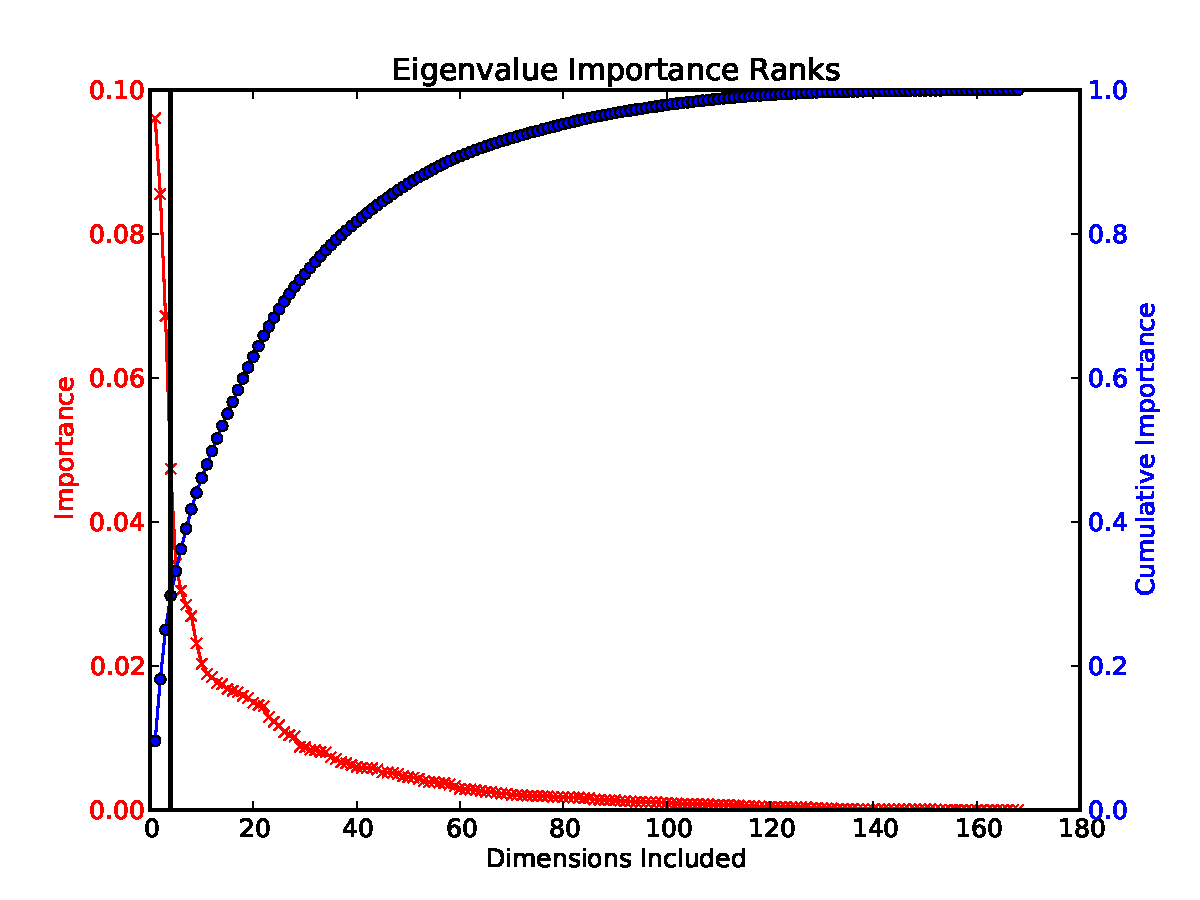
\includegraphics[width=0.7\linewidth]{c5g7/C5G7_eigenvalue_impranks}
  \caption{C5G7 Eigenvalue Importance Ranking}
  \label{fig:c5g7 eigenvalue imprank}
\end{figure}
\begin{figure}[H]
  \centering
  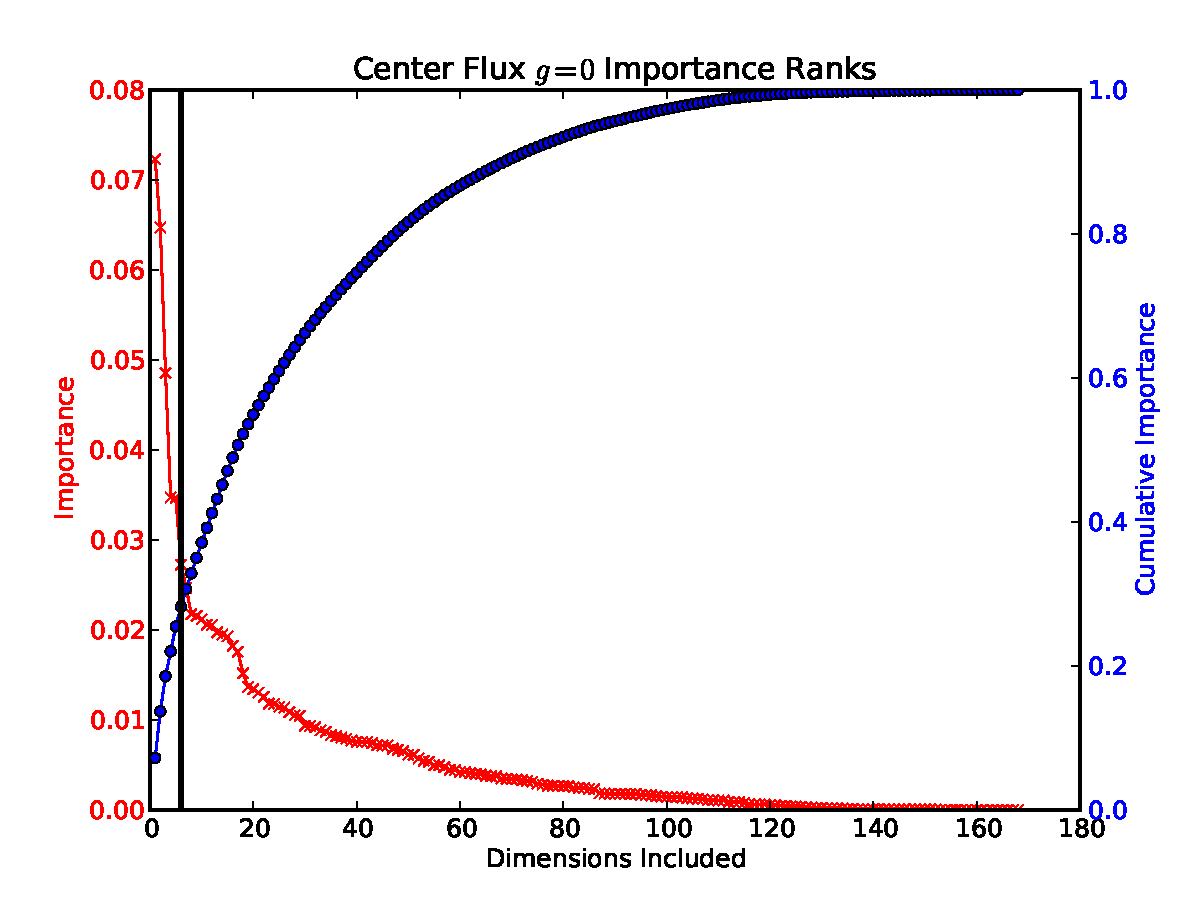
\includegraphics[width=0.7\linewidth]{c5g7/C5G7_center_flux_0_impranks}
  \caption{C5G7 Center Flux ($g=1$) Importance Ranking}
  \label{fig:c5g7 flux 0 imprank}
\end{figure}
\begin{figure}[H]
  \centering
  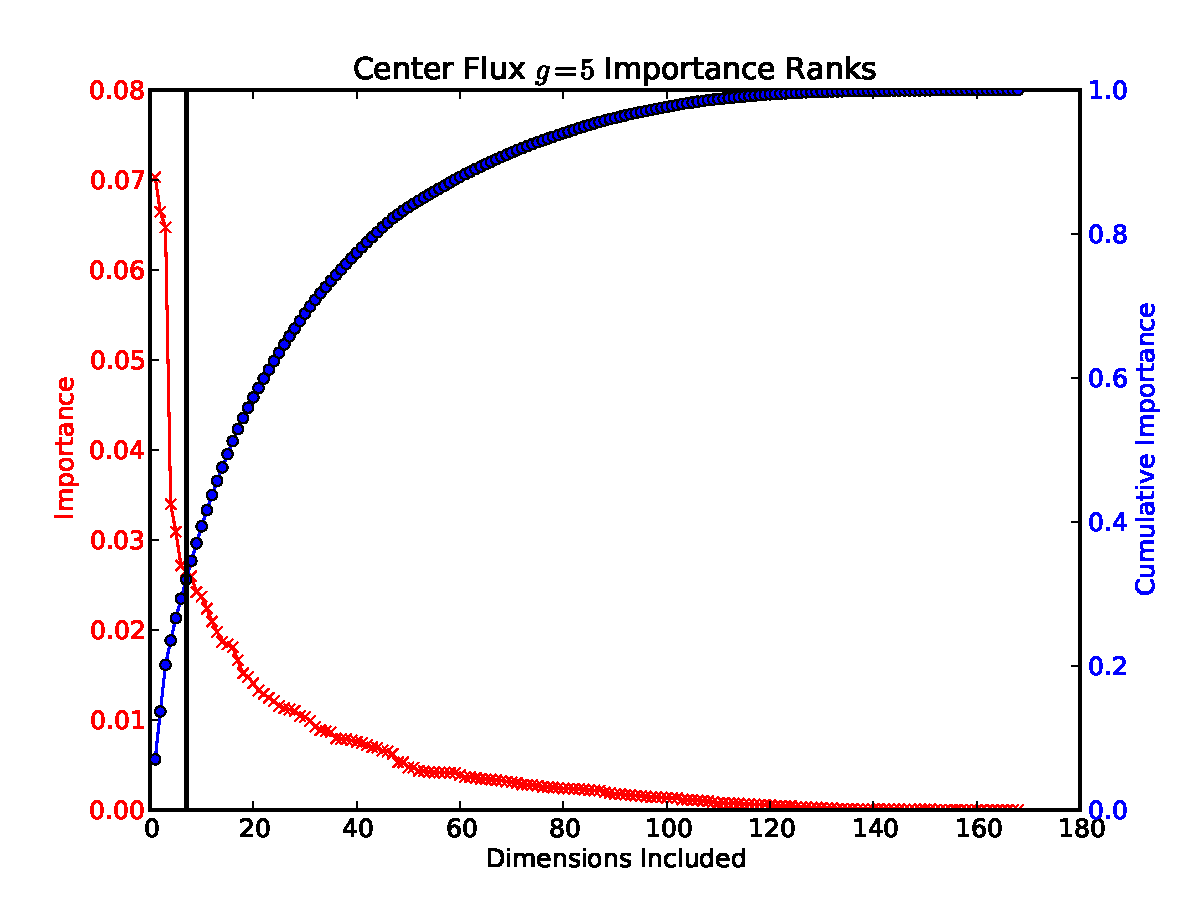
\includegraphics[width=0.7\linewidth]{c5g7/C5G7_center_flux_5_impranks}
  \caption{C5G7 Center Flux ($g=5$) Importance Ranking}
  \label{fig:c5g7 flux 5 imprank}
\end{figure}

The agreement for the mean and standard deviation of the original full input space and the truncated latent
space are shown in Figures \ref{fig:c5g7 eigenvalue red mean} through \ref{fig:c5g7 center_flux_g5 red stdev}.
In each of these figures, the plot on the left shows the process of ten thousand Monte Carlo samples on either
the mean or the standard deviation.  The blue square series is MC on the original, untruncated space, while the red
crosses is MC on the truncated space.  The plot on the right shows the agreement level at ten thousand Monte
Carlo runs.  For the nearly-matching means, the plots are cropped near the calculated values.  For the
poorly-matching standard deviation, we scale the range to demonstrate the portion of the standard deviation
retained. Error bars on both the left and the right plots are given using the mean-based approximation described
in section \ref{sec:res scgpc intro}. 

For all three responses the agreement on the mean values has significant overlap, suggesting the mean was
largely uncompromised by the input space truncation.  The standard deviations, however, do not match as
closely.  For the two flux responses, roughly one quarter of the value was lost due to truncation, while for the
eigenvalue response approximately one fifth of the standard deviation value was lost.  This loss is expected,
as the importance eigenvalues in Table \ref{tab:c5g7 importance} drop off somewhat slowly after the truncation
performed.  With another 12 inputs retained, it is possible to reduce the error in the $k$-eigenvalue
truncation from roughly 25 percent to nearer 10 percent.  However, this truncation is suitable for
demonstration.
\begin{figure}[H]
  \centering
  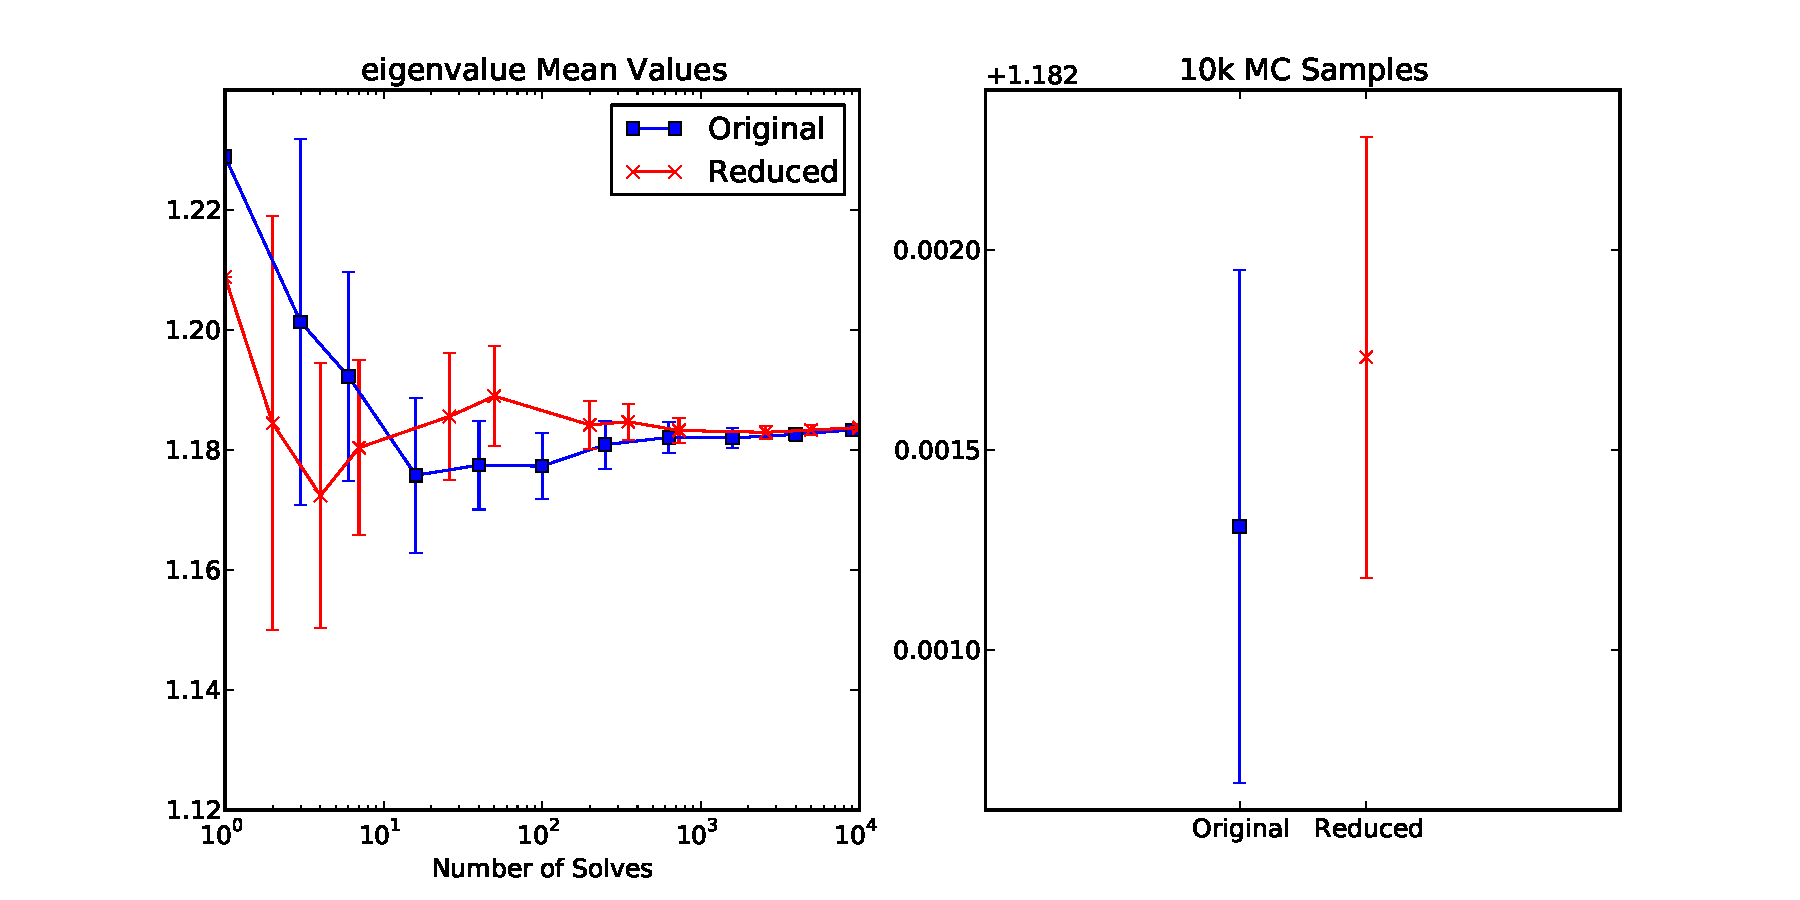
\includegraphics[width=\linewidth]{c5g7/C5G7_eigenvalue_mean_reduction}
  \caption{C5G7 Eigenvalue Input Reduction, Mean}
  \label{fig:c5g7 eigenvalue red mean}
\end{figure}
\begin{figure}[H]
  \centering
  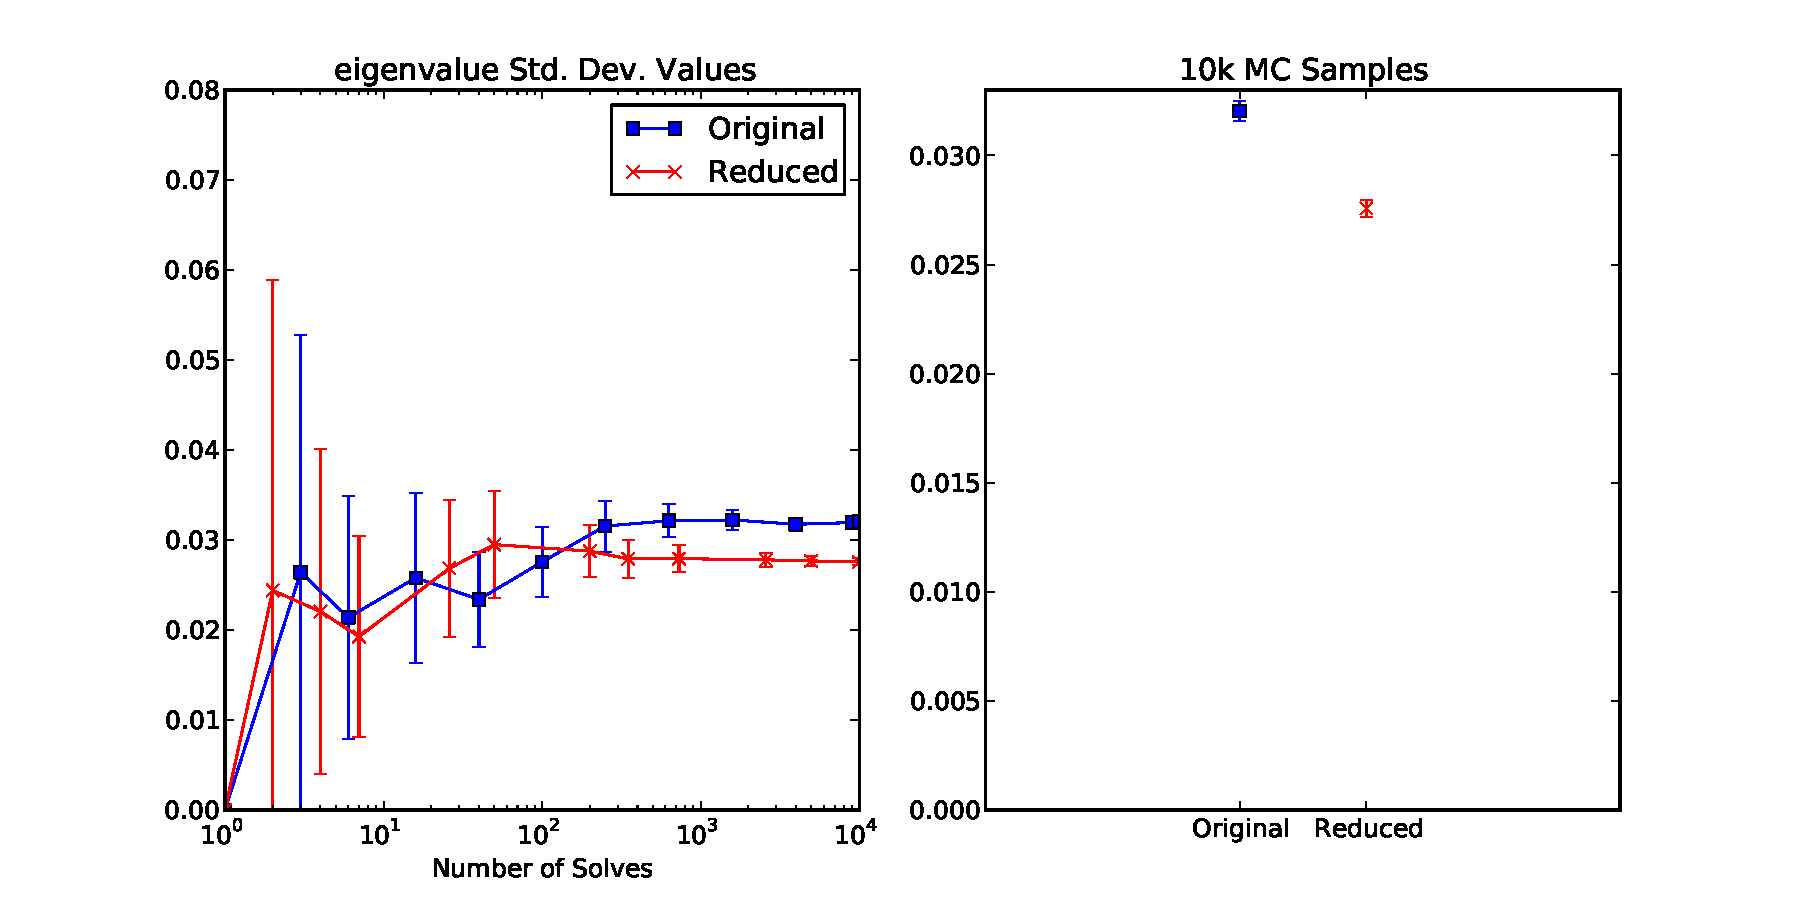
\includegraphics[width=\linewidth]{c5g7/C5G7_eigenvalue_stddev_reduction}
  \caption{C5G7 Eigenvalue Input Reduction, Std. Dev.}
  \label{fig:c5g7 eigenvalue red stdev}
\end{figure}
\begin{figure}[H]
  \centering
  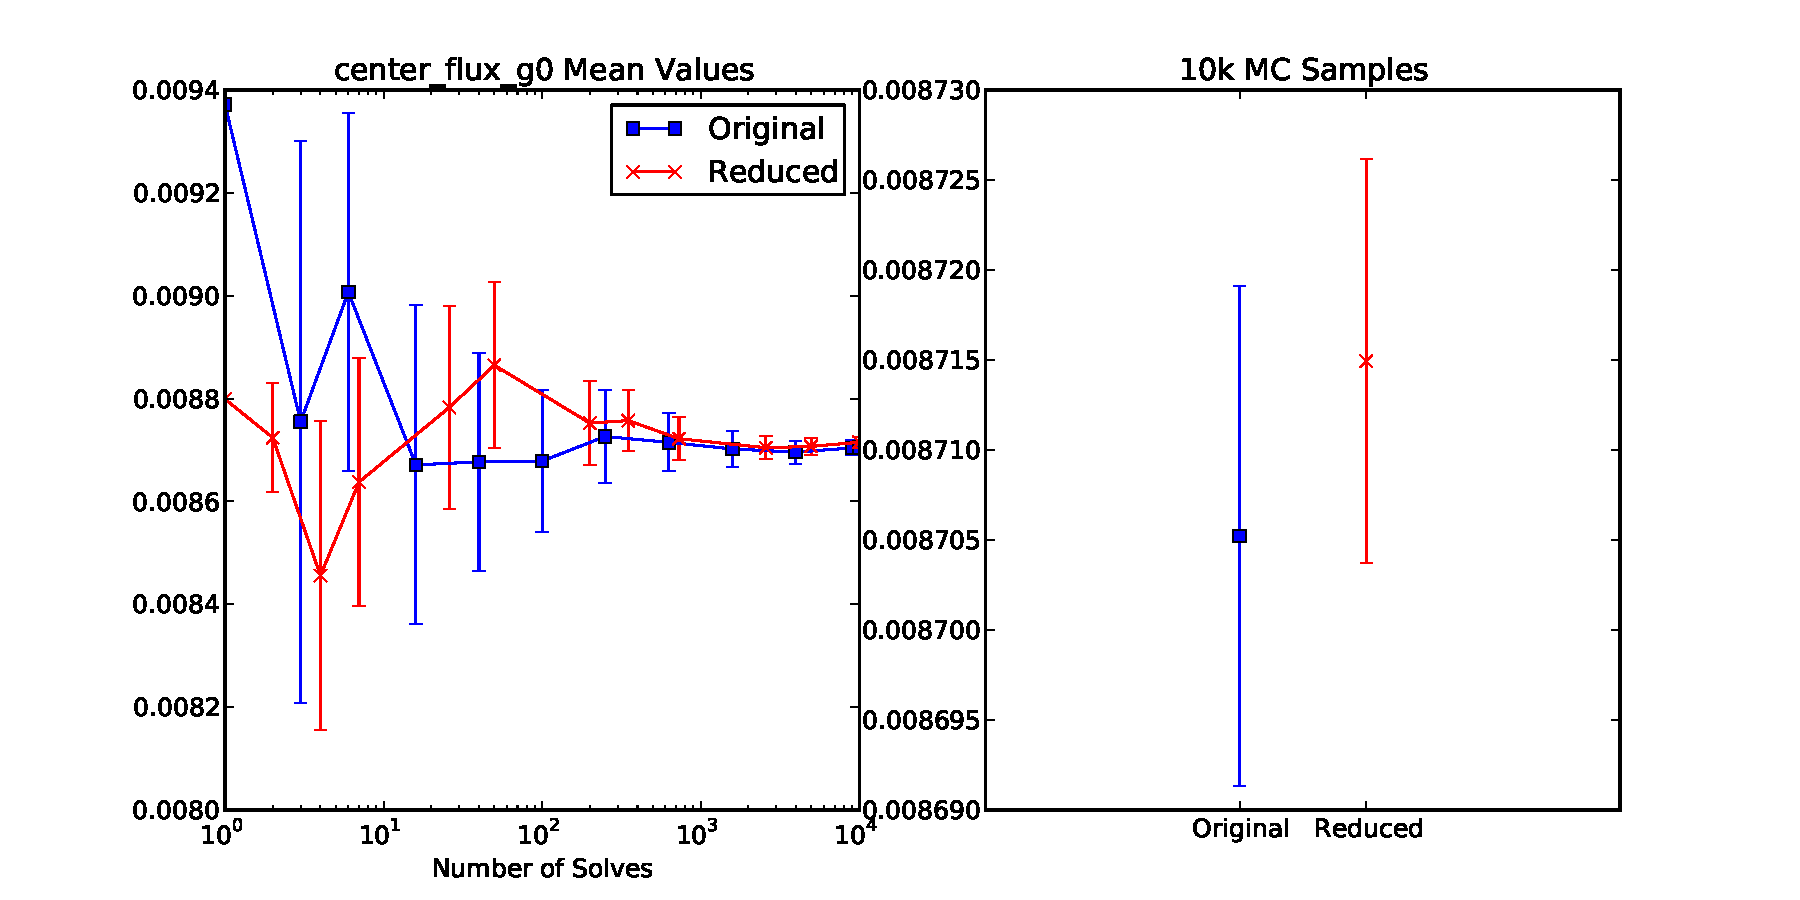
\includegraphics[width=\linewidth]{c5g7/C5G7_center_flux_g0_mean_reduction}
  \caption{C5G7 Center Flux $g=1$ Input Reduction, Mean}
  \label{fig:c5g7 center_flux_g0 red mean}
\end{figure}
\begin{figure}[H]
  \centering
  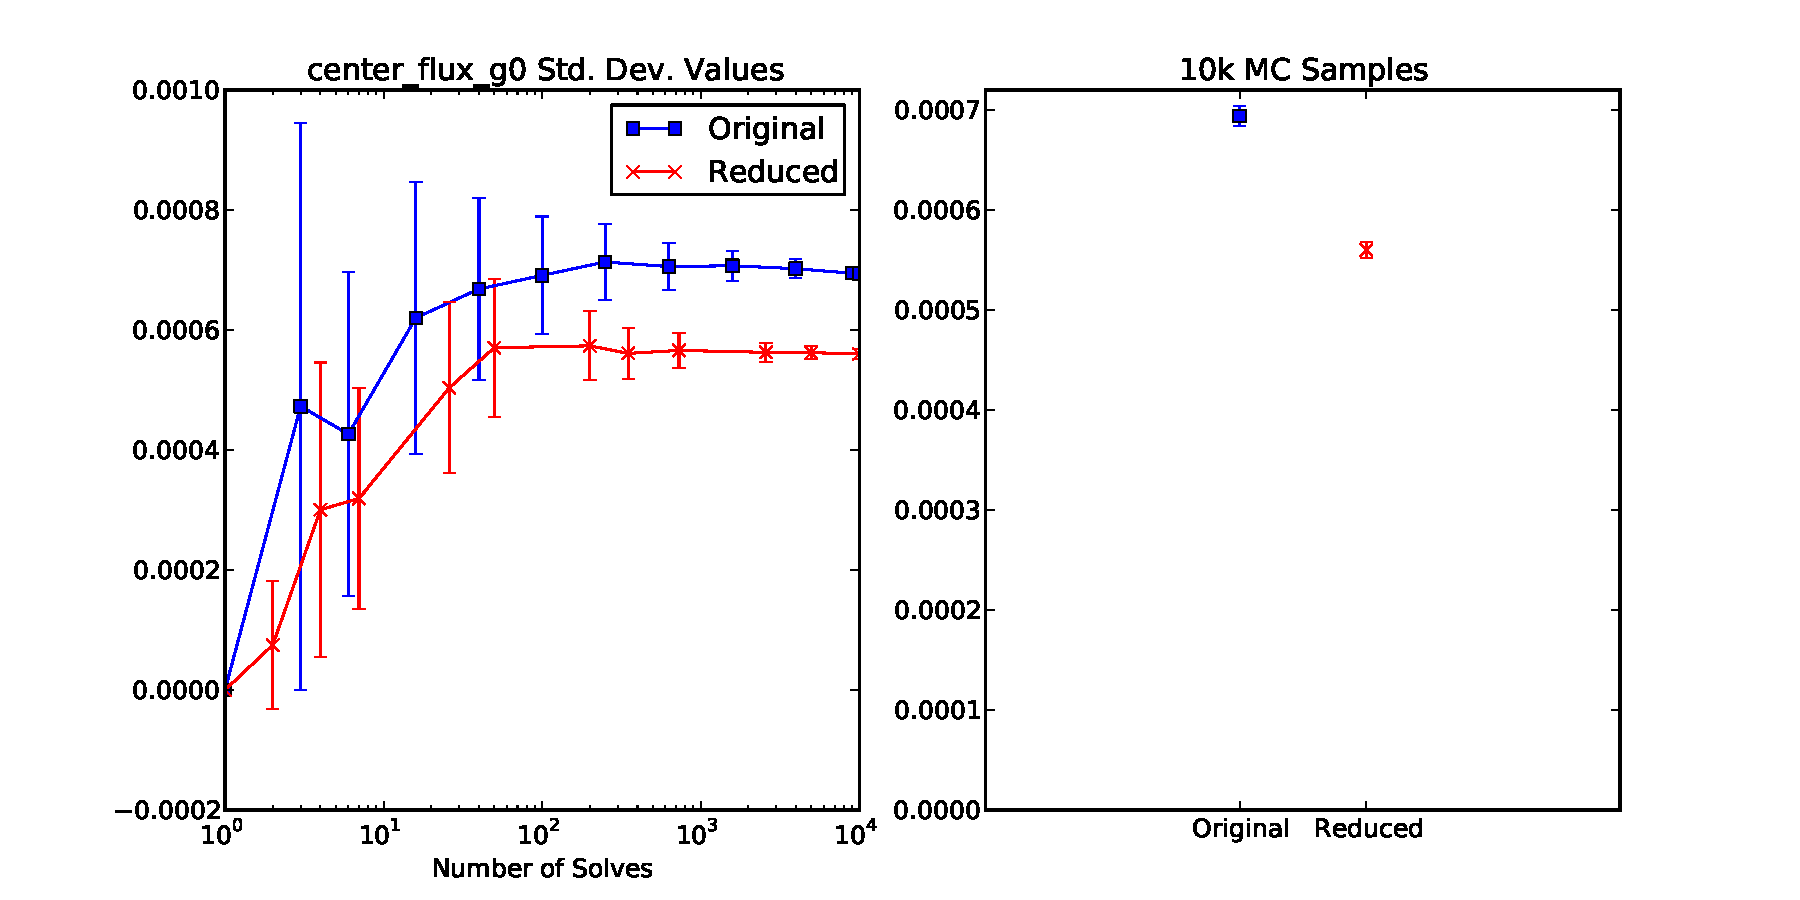
\includegraphics[width=\linewidth]{c5g7/C5G7_center_flux_g0_stddev_reduction}
  \caption{C5G7 Center Flux $g=1$ Input Reduction, Std. Dev.}
  \label{fig:c5g7 center_flux_g0 red stdev}
\end{figure}
\begin{figure}[H]
  \centering
  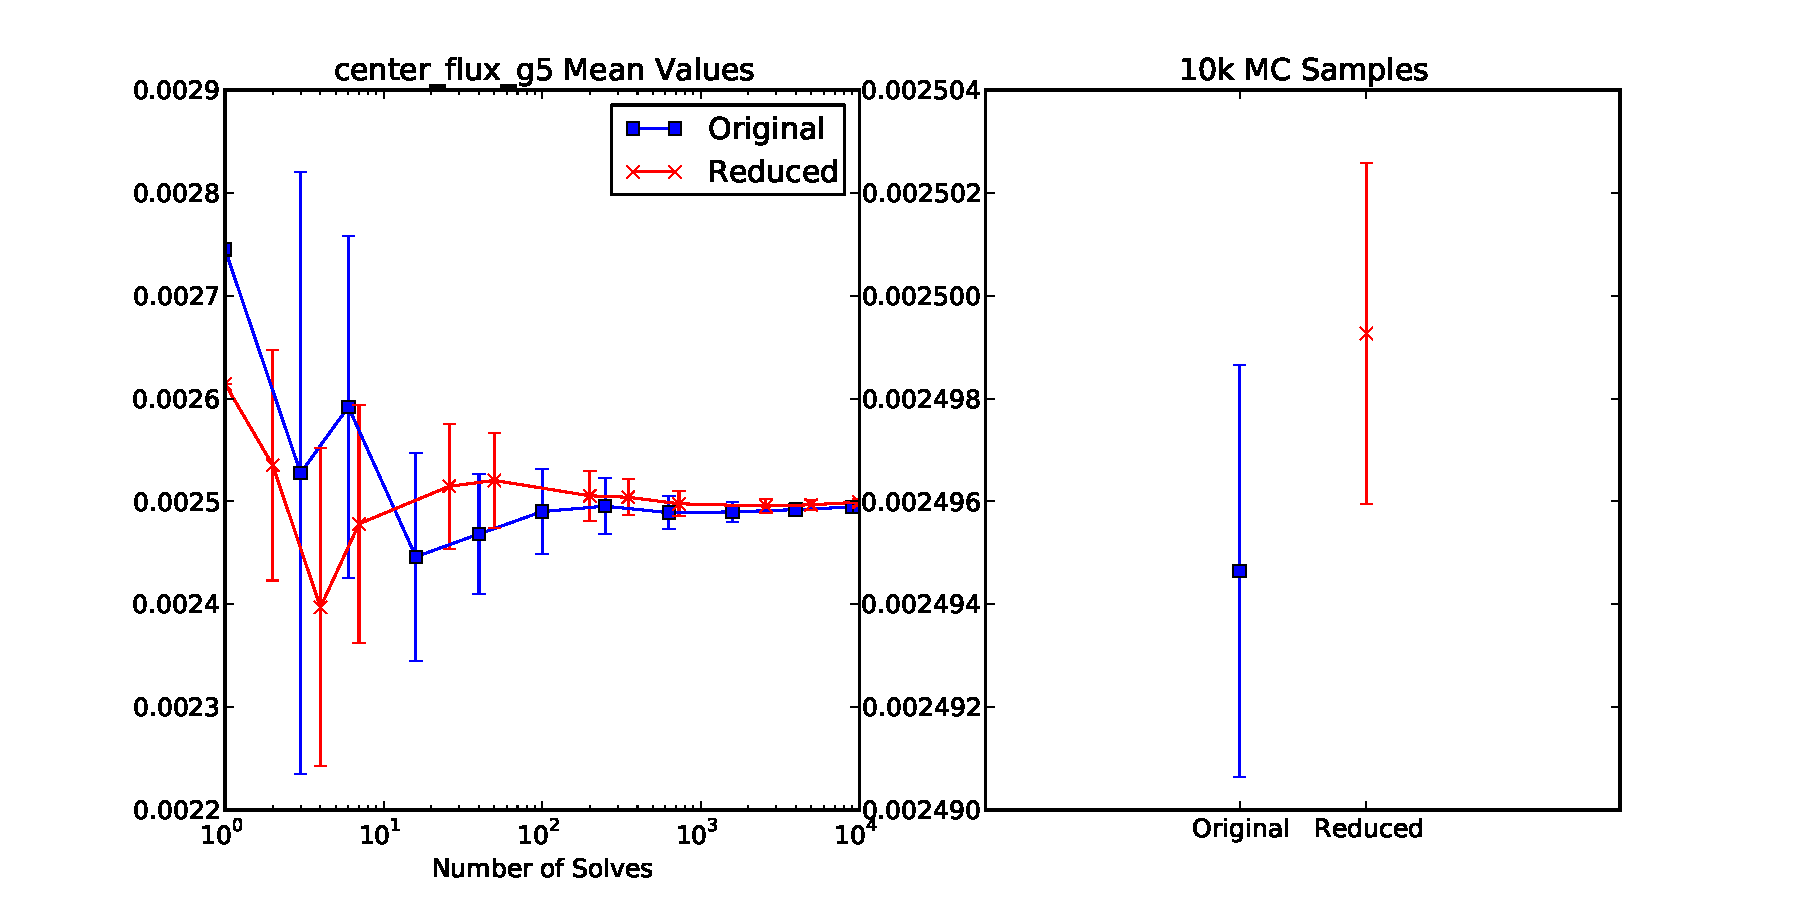
\includegraphics[width=\linewidth]{c5g7/C5G7_center_flux_g5_mean_reduction}
  \caption{C5G7 Center Flux $g=5$ Input Reduction, Mean}
  \label{fig:c5g7 center_flux_g5 red mean}
\end{figure}
\begin{figure}[H]
  \centering
  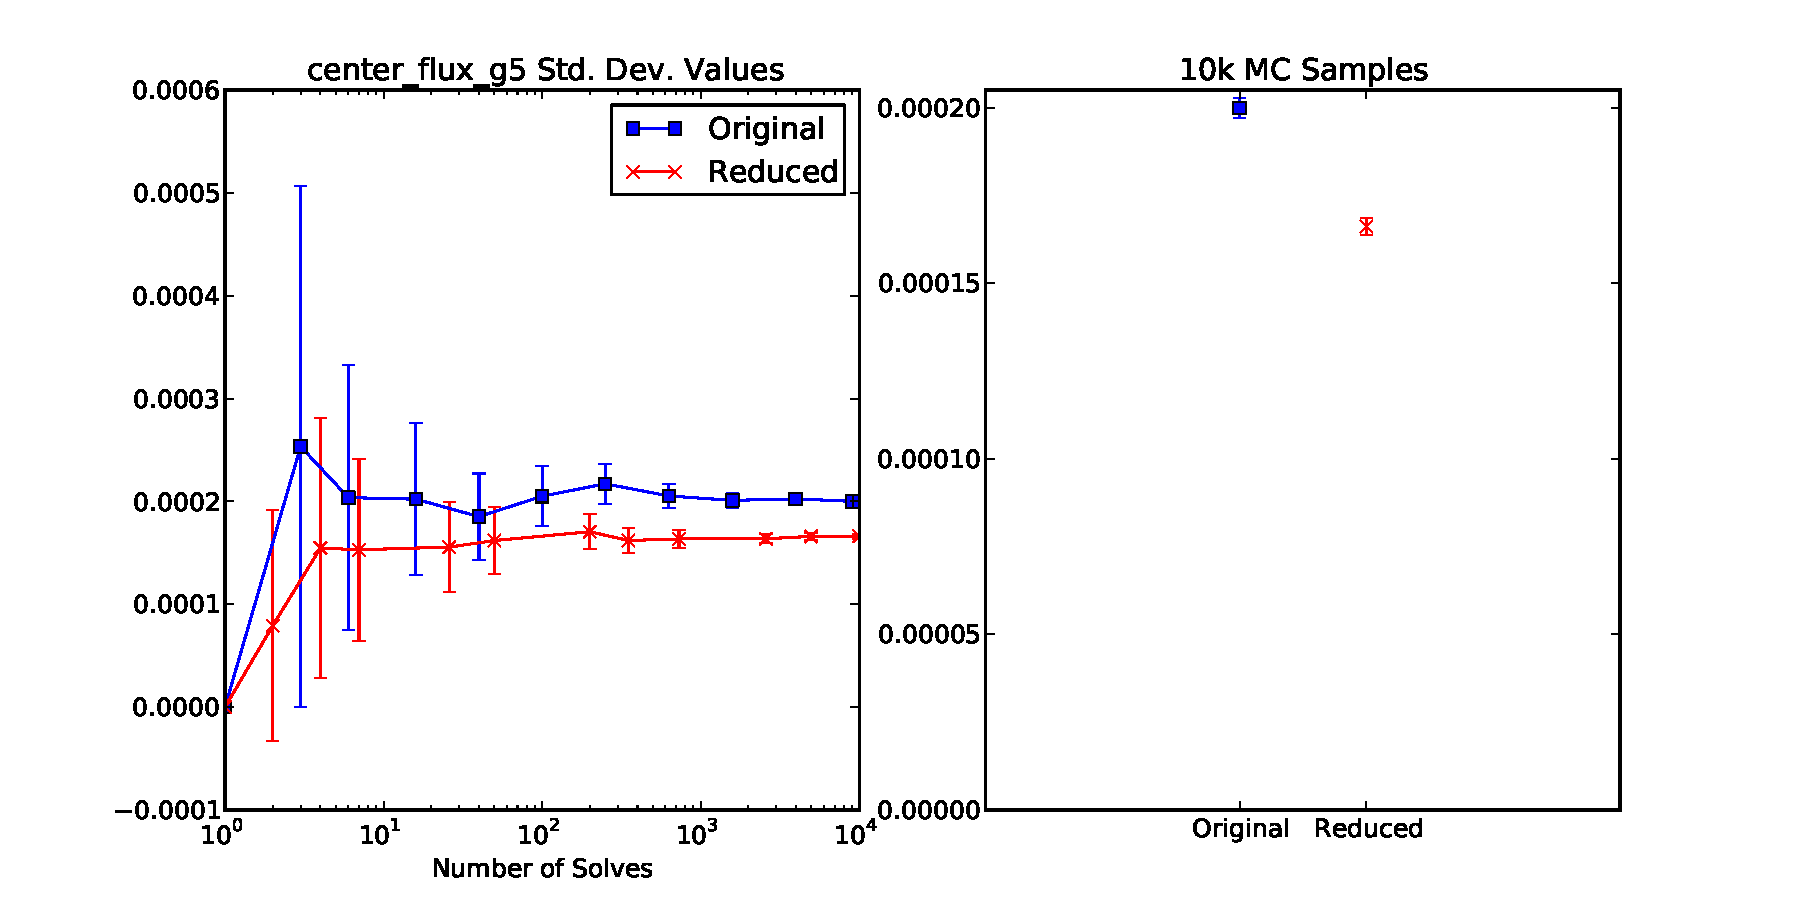
\includegraphics[width=\linewidth]{c5g7/C5G7_center_flux_g5_stddev_reduction}
  \caption{C5G7 Center Flux $g=5$ Input Reduction, Std. Dev.}
  \label{fig:c5g7 center_flux_g5 red stdev}
\end{figure}

Since the efforts in this demonstration are to establish the effectiveness of collocation-based methods for
this model, we consider agreement between collocation expansions and the reduced-space Monte Carlo statistics only.
We ignore the original model statistics and instead consider agreement with the truncated input space.
Comparison to the original model can be done by comparing to the reduced case MC, then comparing reduced space
MC with the original model as we have shown here.

\section{Results}
In general, we observe that no one particular SCgPC or HDMR method stands out as faster converging for the
responses in this model.  All of them converge quite quickly on a solution that is reasonably close to the one
obtained by MC.  While occasionally the converged values are just outside the error bands shown in the plots,
these error bands only guarantee 75 percent certainty (see section \ref{sec:stat moments}).  Thus, we do not
see significant disagreement between the MC values and the SCgPC and HDMR values in these cases.

We also note that in none of the responses does adding additional polynomial affect the predicted mean and
standard deviation from the SCgPC and HDMR methods.  This suggests strong linearity between the responses and
the input parameters, which can be captured by only first-order polynomial expansions.  For this particular
model, the results obtained with under 20 samples with any of the SCgPC or HDMR methods is as good as spending
ten thousand samples using MC.

\subsection{$k$-Eigenvalue}
The performance of SCgPC and HDMR methods for the C5G7 uncertainty quantification problem are shown in Figures
\ref{fig:c5g7 eigenvalue means} and \ref{fig:c5g7 eigenvalue vars}.  All the results shown, including the
Monte Carlo comparison case, are performed with the reduced-size input space.
As seen in the figures, for this response even linear polynomials are sufficient to quite accurately capture the first
two statistical moments of the $k$-eigenvalue.  This suggests a strongly linear dependence of
$k$ on cross sections, which can be justified through analyzing the first derivatives Eq. \ref{eq:diffusion}
with respect to each cross section independently.  This means that any of the collocation methods are very
well-suited to represent the original model, and a cost of far less computational solves than traditional
MC.  Even when scaling the plot to very small ranges, the various collocation-based methods have
indistinguishable values for both the mean and standard deviation.

\begin{figure}[H]
  \centering
  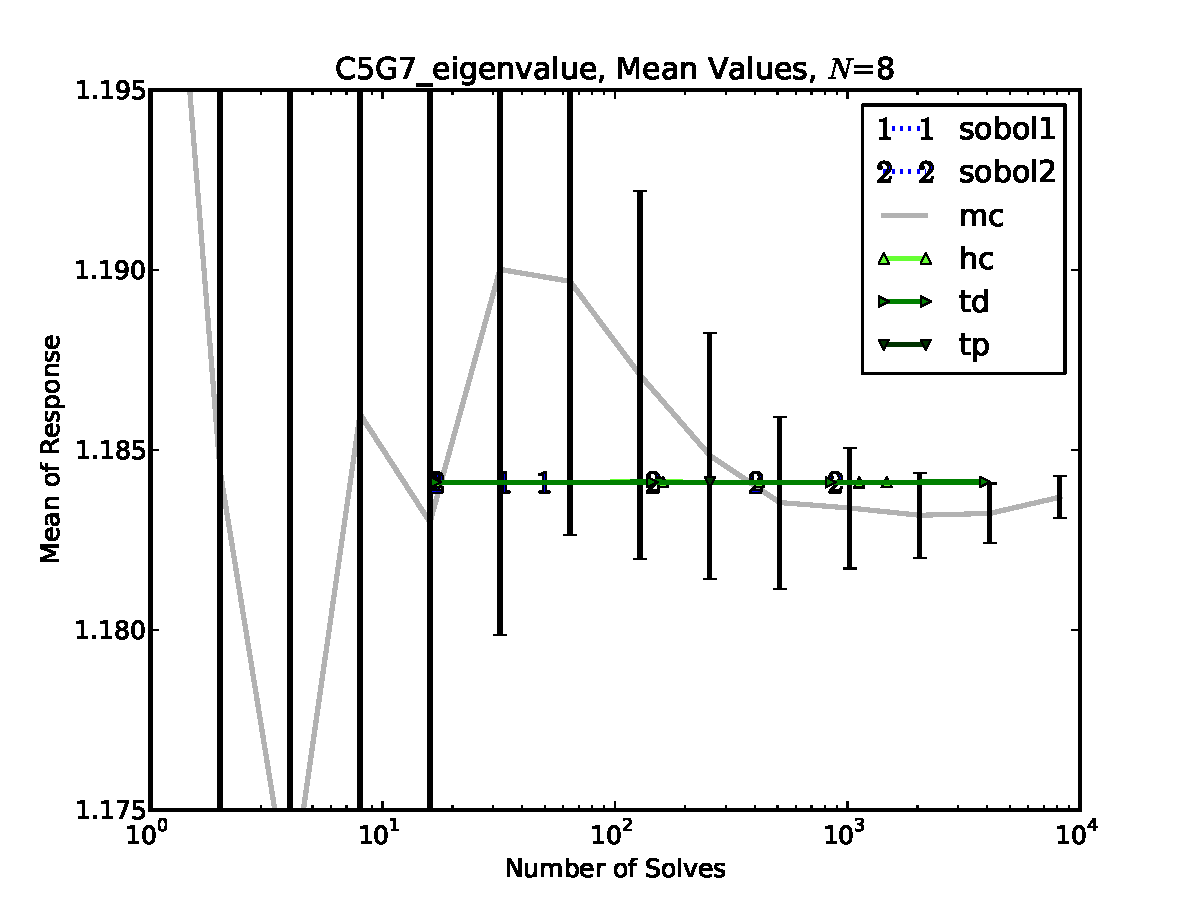
\includegraphics[width=0.7\linewidth]{c5g7/C5G7_eigenvalue_mean_vals}
  \caption{C5G7 $k$-Eigenvalue Mean Values}
  \label{fig:c5g7 eigenvalue means}
\end{figure}
\begin{figure}[H]
  \centering
  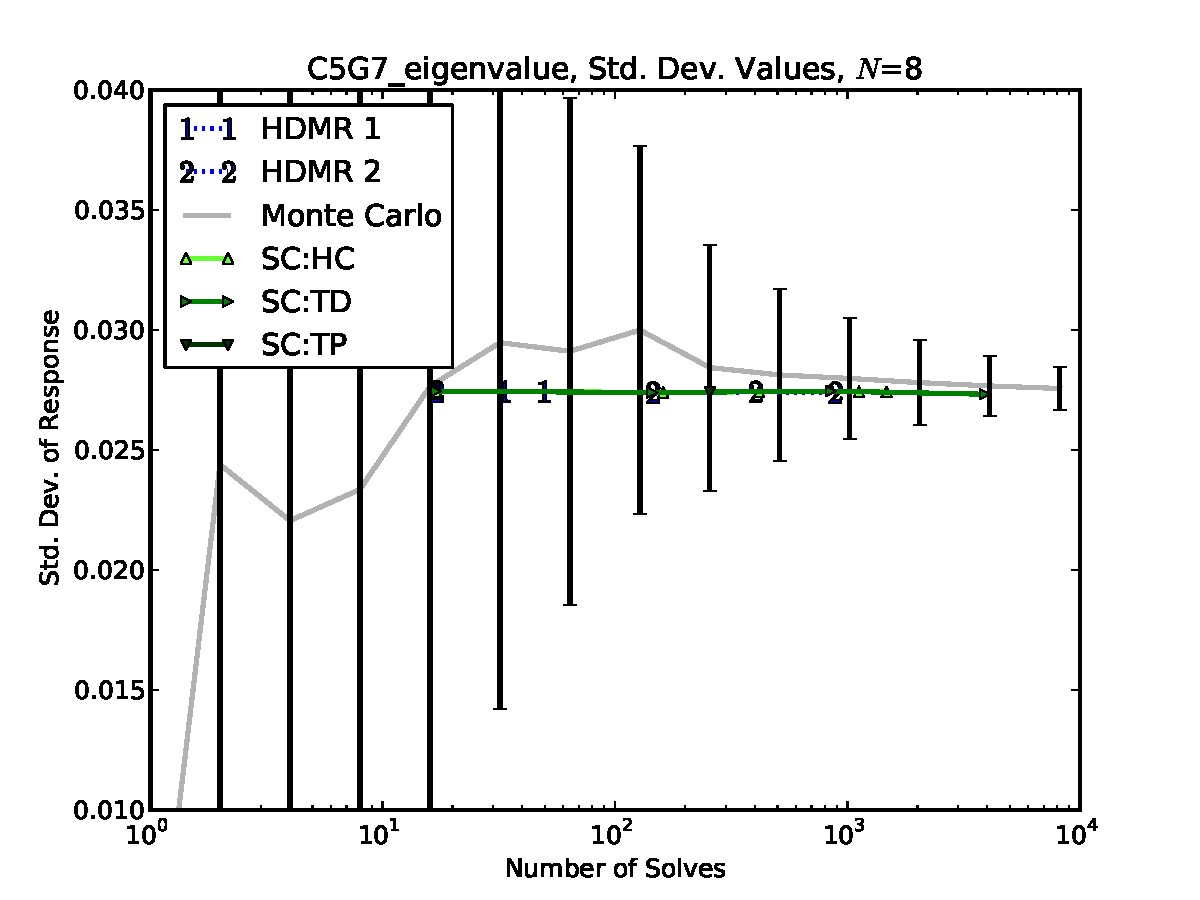
\includegraphics[width=0.7\linewidth]{c5g7/C5G7_eigenvalue_var_vals}
  \caption{C5G7 $k$-Eigenvalue Std. Dev. Values}
  \label{fig:c5g7 eigenvalue vars}
\end{figure}

\subsection{Center Flux, $g=1$}
As with the $k$-eigenvalue, the high-energy flux response appears to be entirely linearly-dependent on the
input parameters.  Adding additional polynomials to any SCgPC or HDMR method does not notably change the
predicted mean or standard deviation.  In the case of the HDMR method, adding pairwise interactions also seems
to have no effect on the predicted response moments.  This suggests the response is not only linear with
respect to the inputs, but that there is little interaction between the inputs when considering the first two
statistical moments of the response.  However, for the standard deviation of this response, there does appear
to be some small amount of shape in the SCgPC and HDMR series, suggesting some level on nonlinearity.

\begin{figure}[H]
  \centering
  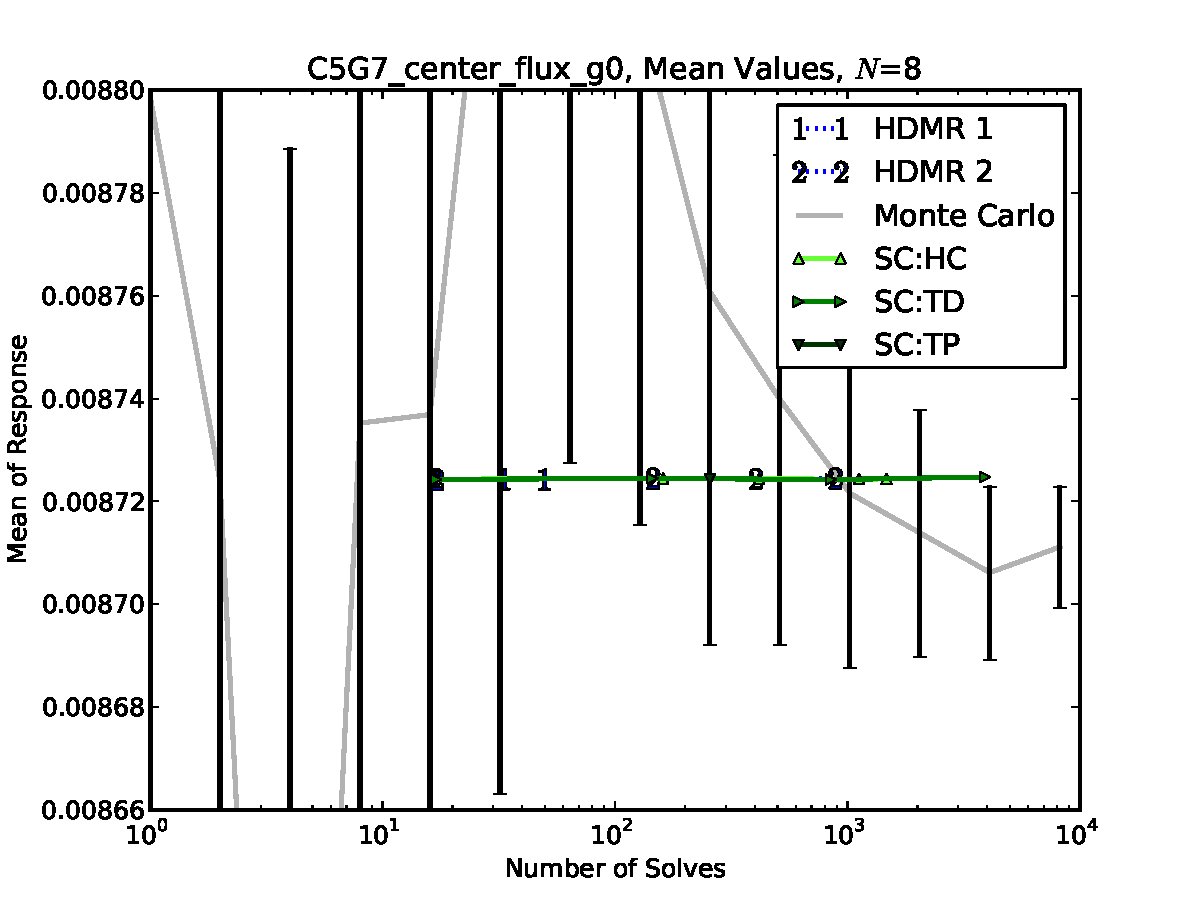
\includegraphics[width=0.7\linewidth]{c5g7/C5G7_center_flux_g0_mean_vals}
  \caption{C5G7 Center Flux $g=1$ Mean Values}
  \label{fig:c5g7 center_flux_g0 means}
\end{figure}
\begin{figure}[H]
  \centering
  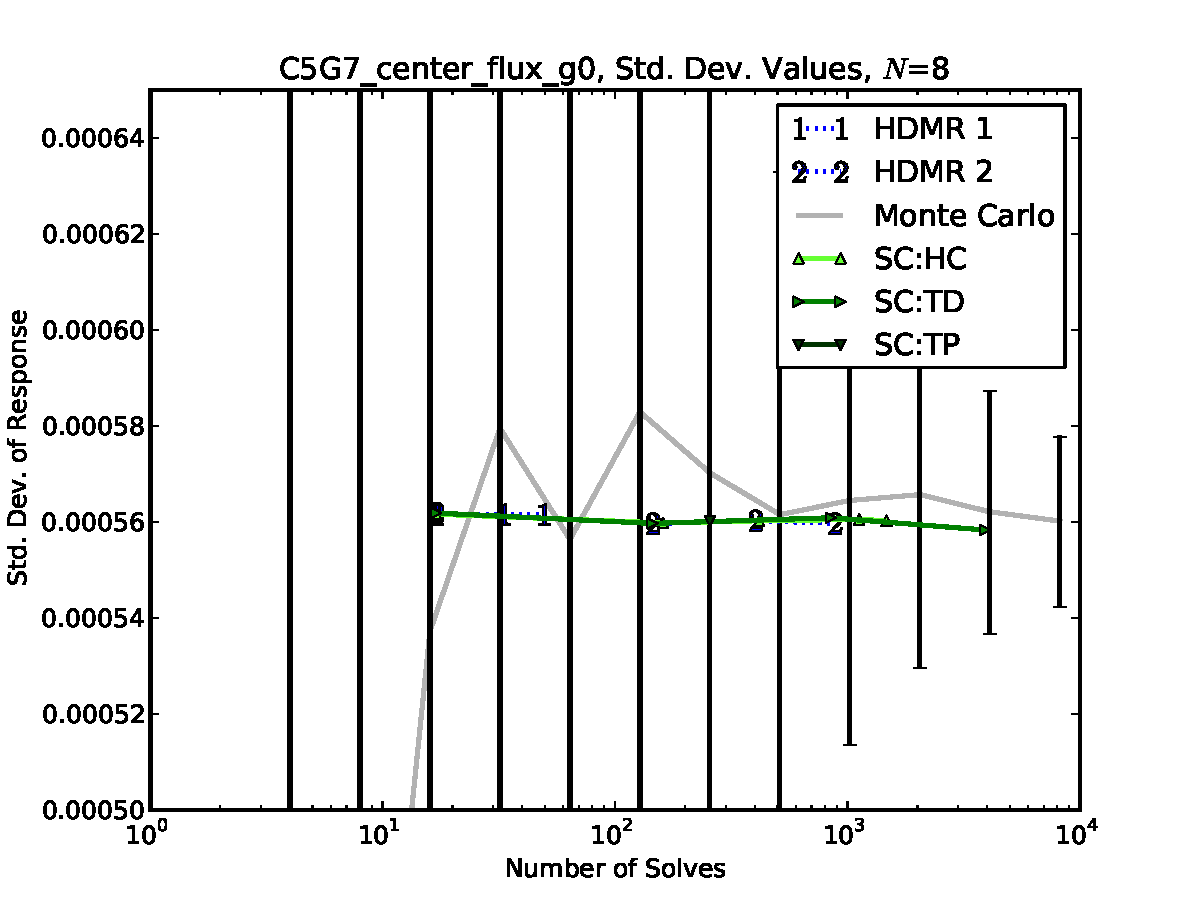
\includegraphics[width=0.7\linewidth]{c5g7/C5G7_center_flux_g0_var_vals}
  \caption{C5G7 Center Flux $g=1$ Std. Dev. Values}
  \label{fig:c5g7 center_flux_g0 vars}
\end{figure}

\subsection{Center Flux, $g=5$}
The low-energy flux demonstrates similar performance to the other two responses.  Whatever nonlinearity
between inputs and the response was present in the high-energy flux standard deviation does not appear to be
present in the low-energy flux.  This seems reasonable, as the mean free path of neutrons in the high-energy
flux is much larger than the low-energy flux, making interaction with many different cross sections in a
variety of ways more likely.  As with the $k$-eigenvalue response, the second-order statistics for the
low-energy flux converge with first-order interactions and first-order polynomials, and show no change
in value after that point.  Both the mean and standard deviation are in good agreement with the estimate
provided by MC.

\begin{figure}[H]
  \centering
  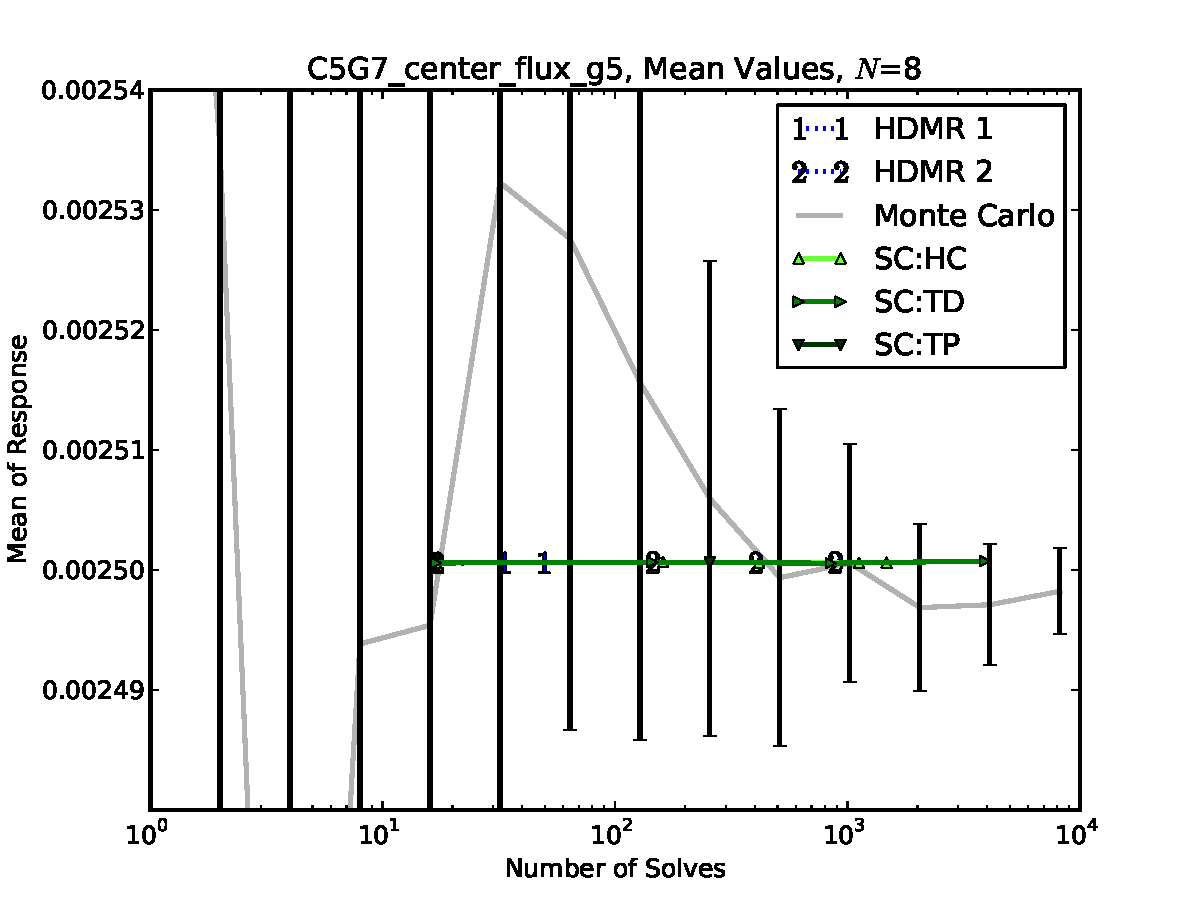
\includegraphics[width=0.7\linewidth]{c5g7/C5G7_center_flux_g5_mean_vals}
  \caption{C5G7 Center Flux $g=5$ Mean Values}
  \label{fig:c5g7 center_flux_g5 means}
\end{figure}
\begin{figure}[H]
  \centering
  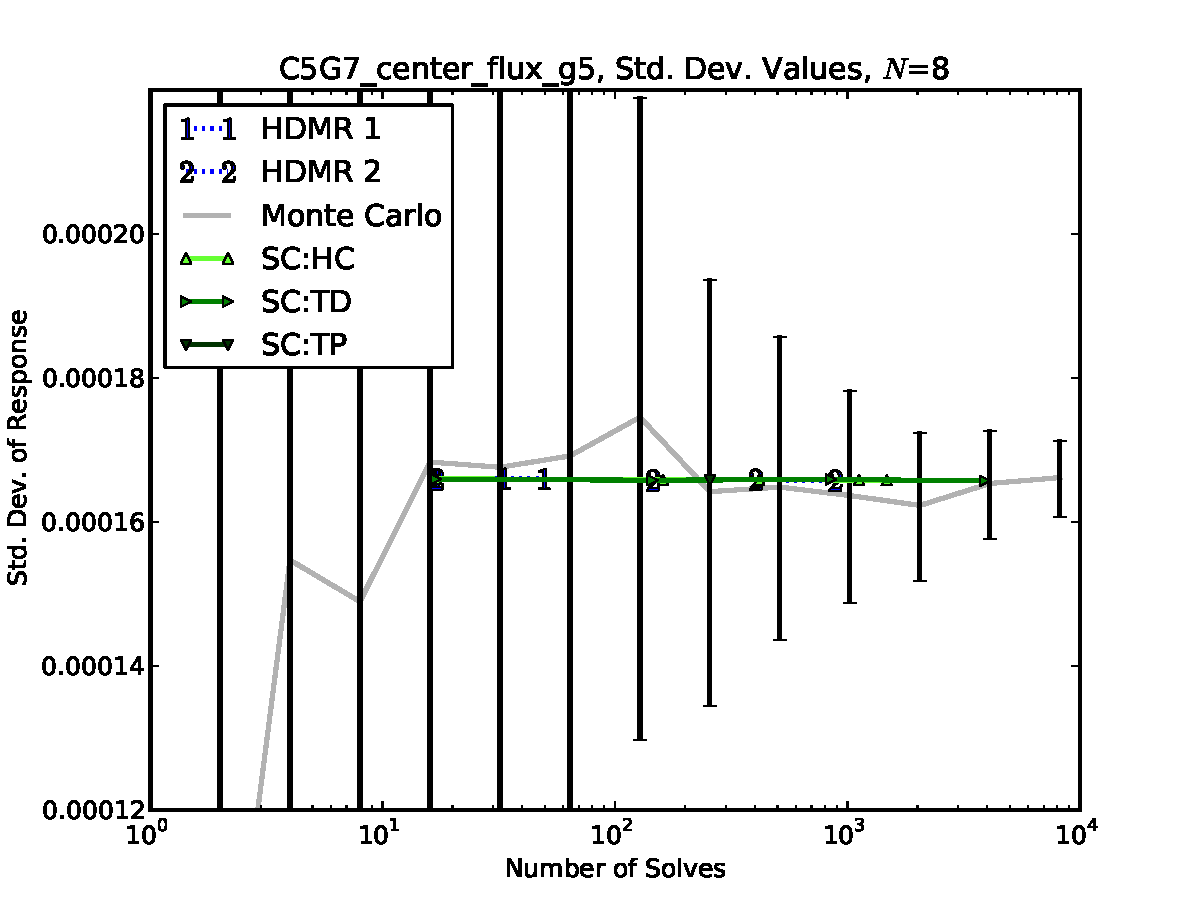
\includegraphics[width=0.7\linewidth]{c5g7/C5G7_center_flux_g5_var_vals}
  \caption{C5G7 Center Flux $g=5$ Std. Dev. Values}
  \label{fig:c5g7 center_flux_g5 vars}
\end{figure}

\section{Conclusion}
Through this model we have explored application of SCgPC and HDMR to responses that are without analytic form
and are solved using an engineering-scale production code.  We observed the methodology for using input space
reduction techniques in order to make collocation-based method more accessible.  We observed that for all
three responses of this model, the SCgPC and HDMR methods both very efficiently converged on statistical
moments in less than 20 computational solves that agreed with MC after ten thousand samples.  For this
particular model and set of responses, SCgPC and HDMR are both excellent uncertainty quantification tools.
